\documentclass[__main__.tex]{subfiles}

\begin{document}

\qtitle{Э}{02}
Гипотеза молекулярных токов Ампера. Теорема о циркуляции вектора $\vec{H}$. Условия на границе раздела магнетиков.\\ 
%%
\textbf{Гипотеза Ампера}\\
Для объяснения намагничения тел Ампер предположил, что в молекулах вещества циркулируют круговые токи. Каждый такой ток обладает магнитным моментом и создаёт в окружающем пространстве магнитное поле. В отсутствие внешнего поля молекулярные токи ориентированы беспорядочным образом, вследствие чего обусловленное ими результирующее поле равно нулю. В силу хаотической ориентации магнитных моментов отдельных молекул суммарный магнитный момент тела также равен нулю. Под действием поля магнитные моменты молекул приобретают преимущественную ориентацию в одном направлении, вследствие чего магнетик намагничивается - его суммарный магнитный момент становится отличным от нуля. Магнитные поля отдельных молекулярных токов в этом случае уже не компенсируют друг друга и возникает поле $\vec{B'}$.
\begin{theorem}[о циркуляции вектора $\vec{H}$]
	Циркуляция вектора напряжённости магнитного поля по некоторому контуру равна алгебраической сумме макроскопических токов, охватываемых этим контуром.
	\begin{gather}
	\oint{H_ldl} = \sum{i},
	\label{e-02-H1}\\
	\oint{H_ldl} = \oint_S{j_ndS},
	\label{e-02-H2}
	\end{gather}
	где 
	$S$ - произвольная поверхность, ограниченная контуром, по которому берётся циркуляция;\\
	$\vec{H} = \frac{B}{\mu_0} - \vec{J}$ - напряжённость магнитного поля;\\
	$i$ - макроскопические токи, охватываемые контуром;\\
	$j_n$ - плотности токов.
\end{theorem}
\begin{proof}
	Вывод формулы - та ещё полотнина. (Савельев.Курс общей физики, том 2. с 143-145).
\end{proof}
\textbf{Условия на границе раздела магнетиков}\\
Вблизи поверхности раздела двух магнетиков векторы $\vec{B}$ и $\vec{H}$ должны удовлетворять определённым граничным условим, которые вытекают из соотношений
\begin{gather}
\nabla B = 0 \hspace{0.3cm} \nabla\times \vec{H} = \vec{j}
\label{e-02-boundary} 
\end{gather}
\begin{wrapfigure}{L}{.3\linewidth}
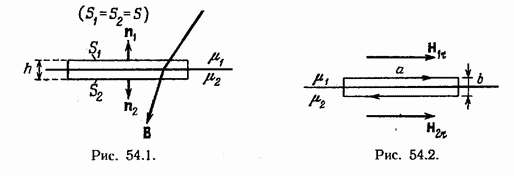
\includegraphics{e-02-1}
\caption{рисунок э-02}
\label{e-02-cylinder}
\end{wrapfigure}
Мы рассматриваем стационарные, т.е. не изменяющиеся со временем поля.\\
Возьмём на границе двух магнетиков с проницаемостями $\mu_1$ и $\mu_2$ воображаемую цилиндрическую поверхность высоты $h$ с основаниями $S_1$ и $S_2$, расположенными по разные стороны поверхности раздела. Поток вектора $\vec{B}$ через эту поверхность равен
\begin{gather}
\Phi_B = B_{1n}S + B_{2n}S + \langle B_n \rangle S_{бок}
\label{e-02-Phib}
\end{gather}
В соответствии с тем, что $\nabla \vec{B} = 0$, поток вектора $\vec{B}$ через любую замкнутую поверхность равен нулю. Приравниваем нулю \ref{e-02-Phib} и сделав переход $h \rightarrow 0$, придём к соотношению $B_{1n} = -B_{2n}$. Если проектировать $\vec{B}_1$ и $\vec{B}_2$ на одну и ту же нормаль, получится условие
\begin{gather*}
B_{1n} = B_{2n}
\end{gather*}
Заменив согласно $\vec{H} = \frac{B}{\mu_0\mu}$ составляющие $\vec{B}$ соответствующими составляющими вектора $\vec{H}$, получим:
\begin{gather*}
\mu_0 \mu_1 H_{1n} = \mu_0 \mu_2 H_{2n}\\
\frac{H_{1n}}{H_{2n}} = \frac{\mu_2}{\mu_1}
\end{gather*}
Вычислим  циркуляцию $\vec{H}$ для прямоугольного контура как на рисунке \ref{e-02-cylinder}. При малых размерах контура циркуляцию можно представить в виде
\begin{gather}
\oint{H_ldl} = H_{1\tau}a - H_{2\tau}a + \langle H_l \rangle 2b
\label{e-02-oint}
\end{gather}
где $\langle H_l \rangle$ - среднее значение $H_l$ на перпендикулярных к границе участках контура. Если по границе раздела не текут макроскопические токи, $\nabla \vec{H}$ в пределах контура будет равна нулю. Поэтому и циркуляция будет равна нулю. Положив выражение \ref{e-02-oint} равным нулю,предельный переход $b \rightarrow 0$, придём к соотношению
\begin{gather*}
H_{1\tau} = H_{2\tau}
\end{gather*}
Опять же заменив составляющие $\vec{H}$ соответствующими составляющими $\vec{B}$, получим:
\begin{gather*}
\frac{B_{1\tau}}{\mu_0\mu_1} = \frac{B_{2\tau}}{\mu_0\mu_2}\\
\frac{B_{1\tau}}{B_{2\tau}} = \frac{\mu_1}{\mu_2}
\end{gather*}
Итак, можно сказать, что при переходе через границу раздела двух магнетиков нормальная составляющая вектора $\vec{B}$ и тангенциальная составляющая вектора $\vec{H}$ изменяются непрерывно. Тангенциальная составляющая вектора $\vec{B}$ и нормальная составляющая вектора $\vec{H}$ при переходе через границу раздела претерпают разрыв. 
\end{document}